%
% File acl2019.tex
%
%% Based on the style files for ACL 2018, NAACL 2018/19, which were
%% Based on the style files for ACL-2015, with some improvements
%%  taken from the NAACL-2016 style
%% Based on the style files for ACL-2014, which were, in turn,
%% based on ACL-2013, ACL-2012, ACL-2011, ACL-2010, ACL-IJCNLP-2009,
%% EACL-2009, IJCNLP-2008...
%% Based on the style files for EACL 2006 by 
%%e.agirre@ehu.es or Sergi.Balari@uab.es
%% and that of ACL 08 by Joakim Nivre and Noah Smith

\documentclass[11pt,a4paper]{article}
\usepackage[hyperref]{acl2019}
\usepackage{times}
\usepackage{latexsym}
\usepackage{amsmath}
\usepackage{fixmath}
\usepackage{url}
\usepackage{graphicx}
\usepackage{booktabs}
\usepackage{mathtools}
\usepackage[export]{adjustbox}

\aclfinalcopy % Uncomment this line for the final submission
\def\aclpaperid{197} %  Enter the acl Paper ID here

%\setlength\titlebox{5cm}
% You can expand the titlebox if you need extra space
% to show all the authors. Please do not make the titlebox
% smaller than 5cm (the original size); we will check this
% in the camera-ready version and ask you to change it back.

\newcommand\BibTeX{B\textsc{ib}\TeX}

\title{Sentiment Classification using Document Embeddings trained with Cosine Similarity}

\author{Tan Thongtan \\
  Department of Computer Engineering \\
  Mahidol University International College \\
  Mahidol University \\
  Thailand \\
  \texttt{tan.thongtan1@gmail.com} \\\And
  Tanasanee Phienthrakul \\
  Department of Computer Engineering \\
  Faculty of Engineering \\
  Mahidol University \\
  Thailand \\
  \texttt{tanasanee.phi@mahidol.ac.th} \\}

\date{}

\begin{document}
\maketitle
\begin{abstract}
In document-level sentiment classification, each document must be mapped to a fixed length vector. Document embedding models map each document to a dense, low-dimensional vector in continuous vector space. This paper proposes training document embeddings using cosine similarity instead of dot product. Experiments on the IMDB dataset show that accuracy is improved when using cosine similarity compared to using dot product, while using feature combination with Naïve Bayes weighted bag of n-grams achieves a new state of the art accuracy of 97.42\%. Code to reproduce all experiments is available at https://github.com/tanthongtan/dv-cosine. 
\end{abstract}

\section{Introduction}



In document classification tasks such as sentiment classification (in this paper we focus on binary sentiment classification of long movie reviews, i.e. determining whether each review is positive or negative), the choice of document representation is usually more important than the choice of classifier. The task of text representation aims at mapping variable length texts into fixed length vectors, as to be valid inputs to a classifier. Document embedding models achieve this by mapping each document to a dense, real-valued vector. 

This paper aims to improve existing document embedding models \cite{le2014,li2016a} by training document embeddings
using cosine similarity instead of dot product. For example, in the basic model of trying to
predict - given a document - the words/n-grams in the document, instead of
trying to maximize the dot product between a document vector
and vectors of the words/n-grams in the document over the training set, we'll be trying to
maximize the cosine similarity instead. 

The motivation behind this is twofold. Firstly, cosine similarity serves as a regularization mechanism; by
ignoring vector magnitudes, there is less incentive to increase the magnitudes of the 
input and output vectors, whereas in the case of dot product, vectors of frequent document-n-gram pairs can be made to have a 
high dot product simply by increasing the magnitudes of each vector. The weights learned should be smaller
overall. 

Secondly, as cosine similarity is widely used to measure document similarity \cite{singhal2001,dai2015}, we believe our
method should more directly maximize the cosine similarity between similar document vectors. The angle
between similar documents should be lower, and that may encode useful information for distinguishing
between different types of documents. We'll compare the performance of our model on the IMDB dataset \cite{maas2011} with
dot product and to determine if our model serves anything beyond simple regularization, we'll also compare
it to dot product using L2 regularization. 

\section{Related Work}


Here we review methods of text representation, in which there are two main categories: \textbf{bag of words models} and \textbf{neural embedding models}. 

The \textbf{bag of words} model \cite{joachims1998} represents text as a fixed length vector of length equal to the number of distinct n-grams in the vocabulary.   
\textbf{Naive Bayes - Support Vector Machine (NB-SVM)} \cite{wang2012} utilizes naïve bayes weighted bag of n-grams vectors for representing texts, feeding these vectors into a logistic regression or support vector machine classifier. 

The first example of a \textbf{neural embedding model} is 
\textbf{word embeddings} which was proposed by \citeauthor{bengio2003} in \citeyear{bengio2003}, while objective functions utilizing the negative sampling technique for efficient training of word embeddings were proposed in \citeyear{mikolov2013} by \citeauthor{mikolov2013} (word2vec). The aim of word embeddings is to map each word to a real vector, whereby the dot product between two vectors represents the amount of similarity in meaning between the words they represent.  
There are two versions of word2vec: continuous bag of words (CBOW), in which a neural network is trained to predict the next word in a piece of text given the word’s context, and skip-gram, where it will try to predict a word’s context given the word itself. 

In a \citeyear{arora2017} paper \citeauthor{arora2017} produce \textbf{Sentence Embeddings} by computing the weighted average of word vectors, where each word is weighted using smooth inverse frequency, and removing the first principle component. 

\textbf{Paragraph Vector} \cite{le2014} may be seen as a modification to word embeddings in order to embed as vectors paragraphs as opposed to words. Paragraph vector comes in two flavors: the Distributed Memory Model of Paragraph Vectors (PV-DM), and the Distributed Bag of Words version of Paragraph Vector (PV-DBOW). 
PV-DM is basically the same as CBOW except that a paragraph vector is additionally averaged or concatenated along with the context and that whole thing is used to predict the next word. 
In the PV-DBOW model a paragraph vector alone is used/trained to predict the words in the paragraph.  

 \textbf{Document Vector by predicting n-grams (DV-ngram)} \cite{li2016a} trains paragraph vectors to predict not only the words in the paragraph, but n-grams in
the paragraph as well. 
  \textbf{Weighted Neural Bag of n-grams  (W-Neural-BON)} \cite{li2016b} uses an objective function similar to the one in DV-ngram, except that each log probability term is weighted using a weighing scheme which is similar to taking the absolute values of naive bayes weights.  

In \cite{li2017}, they introduce three main methods of \textbf{embedding n-grams}. The first is context guided n-gram representation (CGNR), which is training n-gram vectors to predict its context n-grams. The second is label guided n-gram representation (LGNR), which is predicting given an n-gram the label of the document to which it belongs. The last is text guided n-gram representation (TGNR), which is predicting given an n-gram the document to which it belongs. 


\textbf{Embeddings from Language Models (ELMo)} \cite{peters2018} learns contextualized word embeddings by training a bidirectional LSTM \cite{hochreiter1997} on the language modelling 
task of predicting the next word as well as the previous word.
\textbf{Bidirectional Encoder Representations from Transformers (BERT)} \cite{devlin2018} uses the masked language model objective, which is predicting the masked word
given the left and right context, in order to pre-train a multi-layer bidirectional Transformer \cite{vaswani2017}. BERT also jointly pre-trains text-pair
representations by using a next sentence prediction objective. 


For the rest of this section we'll look at other research which replaces dot product with cosine similarity. 
In the context of fully-connected neural networks and convolutional neural networks, \cite{luo2017} uses cosine similarity instead of dot product in computing a layer’s pre-activation as a regularization mechanism. 
Using a special dataset where each instance is a paraphrase pair, \cite{wieting2015} trains word vectors in such a way that the cosine similarity between the resultant document vectors of a paraphrase pair is directly maximized. 

\section{Proposed Model}

In learning neural n-gram and document embeddings, a dot product between the input vector and the output vector is generally
used to compute the similarity measure between the two vectors, i.e. ‘similar’ vectors should have a high dot product. 
In this paper we explore using cosine similarity instead of dot product in computing the similarity measure between the input and output vectors. More specifically we focus on modifications to the PV-DBOW and the similar DV-ngram models. The cosine similarity between a paragraph vector and vectors of n-grams in the paragraph is maximized over the training set. 

\subsection{Architecture}

A neural network is trained to be useful in predicting, given a document, the words and n-grams in the document, in the process of doing so learning useful document embeddings. Formally, the objective function to be minimized is defined as follows:
\begin{equation}
\sum_{d \in D} \sum_{w_o \in W_d} - \log p(w_o | d) \label{eq1}
\end{equation}
where $d$ is a document, $D$ is the set of all documents in the dataset, $w_o$ is an n-gram and $W_d$ is the set of all n-grams in the document $d$. $p(w_o | d)$ is defined using softmax:
\begin{align}
p(w_o | d) &= \frac{e^{\alpha \cos \theta_{w_o}} } {\sum_{w \in W} e^{\alpha \cos \theta_w} } \label{eq2}\\
&= \operatorname{softmax}(\alpha \cos \theta_{w_o}) 
\end{align}
We have $\cos \theta_w$ defined as follows:
\begin{equation}
\cos \theta_w = \frac {\mathbold{v}_d^T \mathbold{v}_w} {\lVert \mathbold{v}_d \rVert \lVert \mathbold{v}_w \rVert}
\end{equation}
where $\mathbold{v}_d$ and $\mathbold{v}_w$ are vector representations of the document $d$ and the word/n-gram $w$ respectively and are parameters to be learned. $\alpha$ is a hyperparameter. $W$ is the set of all n-grams in the vocabulary.

Normally, the softmax of the dot product between the input and output vector is used to model the conditional probability term as follows:
\begin{equation}
p(w_o | d) = \frac{e^{\mathbold{v}_d^T \mathbold{v}_{w_o}} } {\sum_{w \in W} e^{\mathbold{v}_d^T \mathbold{v}_w} }
\end{equation} 
Whereas dot product ranges from negative infinity to positive infinity, since cosine similarity ranges
from -1 to 1, using the cosine similarity term alone as an input to the softmax function may not be sufficient in modeling the conditional probability distribution. Therefore, we add a scaling hyperparameter $\alpha$ to increase the range of possible probability values for each conditional probability term. 

\begin{figure}[h]
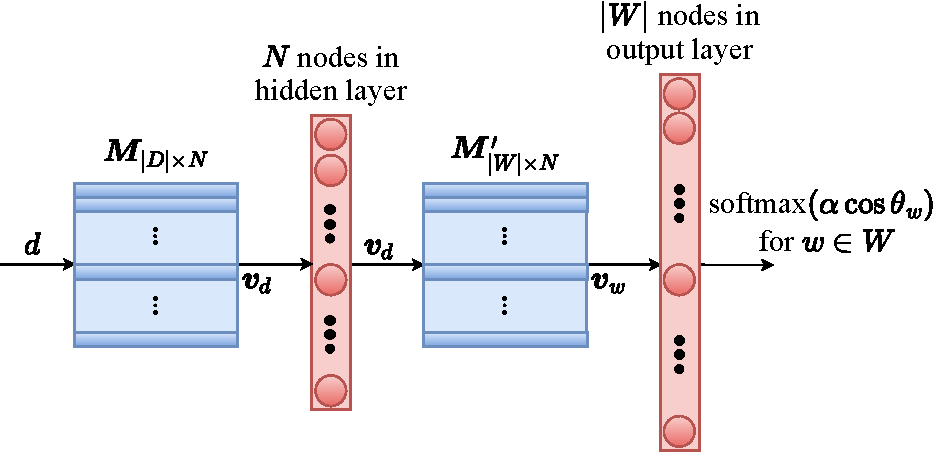
\includegraphics[width=1.02\linewidth,right]{architecture.pdf}
\caption{Proposed Architecture.}
\label{architecture}
\end{figure}

Figure~\ref{architecture} shows the architecture of the neural network used in learning the document embeddings. There is a hidden layer with $N$ nodes corresponding to the dimensionality of the paragraph vectors and an output layer with $\lvert W \rvert$ nodes corresponding to the number of distinct n-grams found in the dataset. There are two weight parameter matrices to be learned: $\mathbold{M}$, which may be seen as a collection of $\lvert D \rvert$ document vectors each having $N$ dimensions, and $\mathbold{M}'$, which is a collection of $\lvert W \rvert$ n-gram vectors each also having $N$ dimensions. 



An input document id $d$ is used to select its vector representation $\mathbold{v}_d$ which is exactly output through the $N$ nodes of the first hidden layer.  The output of each node in the output layer represents the probability $p(w|d)$ of its corresponding n-gram $w$, and is calculated as in \eqref{eq2} using softmax.

\subsection{Negative Sampling}

\setlength{\tabcolsep}{8pt}
\begin{table*}[t]
	\centering
	\small
	\begin{tabular}{@{\hskip6pt}lrrr@{\hskip6pt}}
		\toprule
		Features & Dot Product  & Dot Product &Cosine \\ 
		& (DV-ngram)  &with L2R &   Similarity\\
		&  (\%)& (\%)&   (\%) \\
		\midrule
		Unigrams & 89.60 & 87.15 (-2.45) & \bf{90.75 (+1.15)}  \\
		Unigrams+Bigrams & 91.27 & 91.72 (+0.45) & \bf{92.56 (+1.29)} \\
		Unigrams+Bigrams+Trigrams& 92.14  &92.45 (+0.31) & \bf{93.13 (+0.99)} \\
		\bottomrule
	\end{tabular}
	\caption{Experimental Results.}
	\label{er}
\end{table*}

Since the weight update equations for minimizing \eqref{eq1} implies that we must update each output vector corresponding to each feature in the feature set $W$, with extremely large vocabularies, this computation is impractical. In \cite{mikolov2013}, the negative sampling technique is introduced as a means to speed up the learning process and it can be shown that the updates for the negative sampling version of \eqref{eq1} as shown in \eqref{eq5} approximates the weight updates carried out in minimizing \eqref{eq1}. Therefore in practice, the document embeddings are obtained by minimizing the following objective function with stochastic gradient descent and backpropagation \cite{rumelhart1986}: 
\begin{align}
\sum_{d \in D} \sum_{w_o \in W_d} \biggl[ &- \log \sigma \left( \alpha \cos \theta_{w_o} \right) \nonumber \\
&- \sum_{w_n \in W_{neg}} \log \sigma \left( - \alpha \cos \theta_{w_n} \right) \biggr] \label{eq5}
\end{align}
where $W_{neg}$ is a set of negatively sampled words;
the size of the set or the negative sampling size as
well as the distribution used to draw negatively
sampled words/n-grams are hyperparameters. $\sigma$ is
the sigmoid function. 

By contrast, in the case of dot product the objective function is:
\begin{align}
\sum_{d \in D} \sum_{w_o \in W_d} \biggl[ &- \log \sigma \left( \mathbold{v}_d^T \mathbold{v}_{w_o} \right) \nonumber \\
&- \sum_{w_n \in W_{neg}} \log \sigma \left( - \mathbold{v}_d^T \mathbold{v}_{w_n} \right) \biggr] \label{eqdp}
\end{align}
while in the case of L2R dot product, the objective function used is:
\begin{align}
\sum_{d \in D} &\sum_{w_o \in W_d} \biggl[ - \log \sigma \left( \mathbold{v}_d^T \mathbold{v}_{w_o} \right) + \frac{\lambda}{2}\lVert \mathbold{v}_d \rVert^2 + \frac{\lambda}{2}\lVert \mathbold{v}_{w_o} \rVert^2 \nonumber \\
&- \sum_{w_n \in W_{neg}} \left( \log \sigma \left( - \mathbold{v}_d^T \mathbold{v}_{w_n} \right) + \frac{\lambda}{2}\lVert \mathbold{v}_{w_n} \rVert^2 \right) \biggr] \label{eql2r}
\end{align}
where  $\lambda$ is the regularization strength.

\section{Experiments}



The models are benchmarked on the IMDB dataset \cite{maas2011}, which contains 25,000 training documents, 25,000 test documents, and 50,000 unlabeled documents. The IMDB dataset is a binary sentiment classification dataset consisting of movie reviews retrieved from IMDB; training documents in the dataset are highly polar. For labeled documents, there is a 1:1 ratio between negative and positive documents. The document vectors are learned using all the documents in the dataset (train, test and unlabeled documents). The dataset consists of mainly long movie reviews. 

In order to train the document vectors on unigrams to trigrams, the reviews are preprocessed in such a way that tokens representing bigrams and trigrams are simply appended to the original unigrams of the review itself. An L2-regularized logistic regression (LR) classifier is used to classify the documents at the end of each epoch using the predefined train-test split. However, the results reported in this paper
include only the accuracy obtained from classifying documents in the final epoch. For any java implementations of the LR classifier we use the LIBLINEAR library \cite{fan2008} while for python implementations we use Sci-kit learn \cite{pedregosa2011}. Code to reproduce all experiments is available at https://github.com/tanthongtan/dv-cosine. 




\subsection{Optimal Hyperparameters}

\begin{figure*}[]
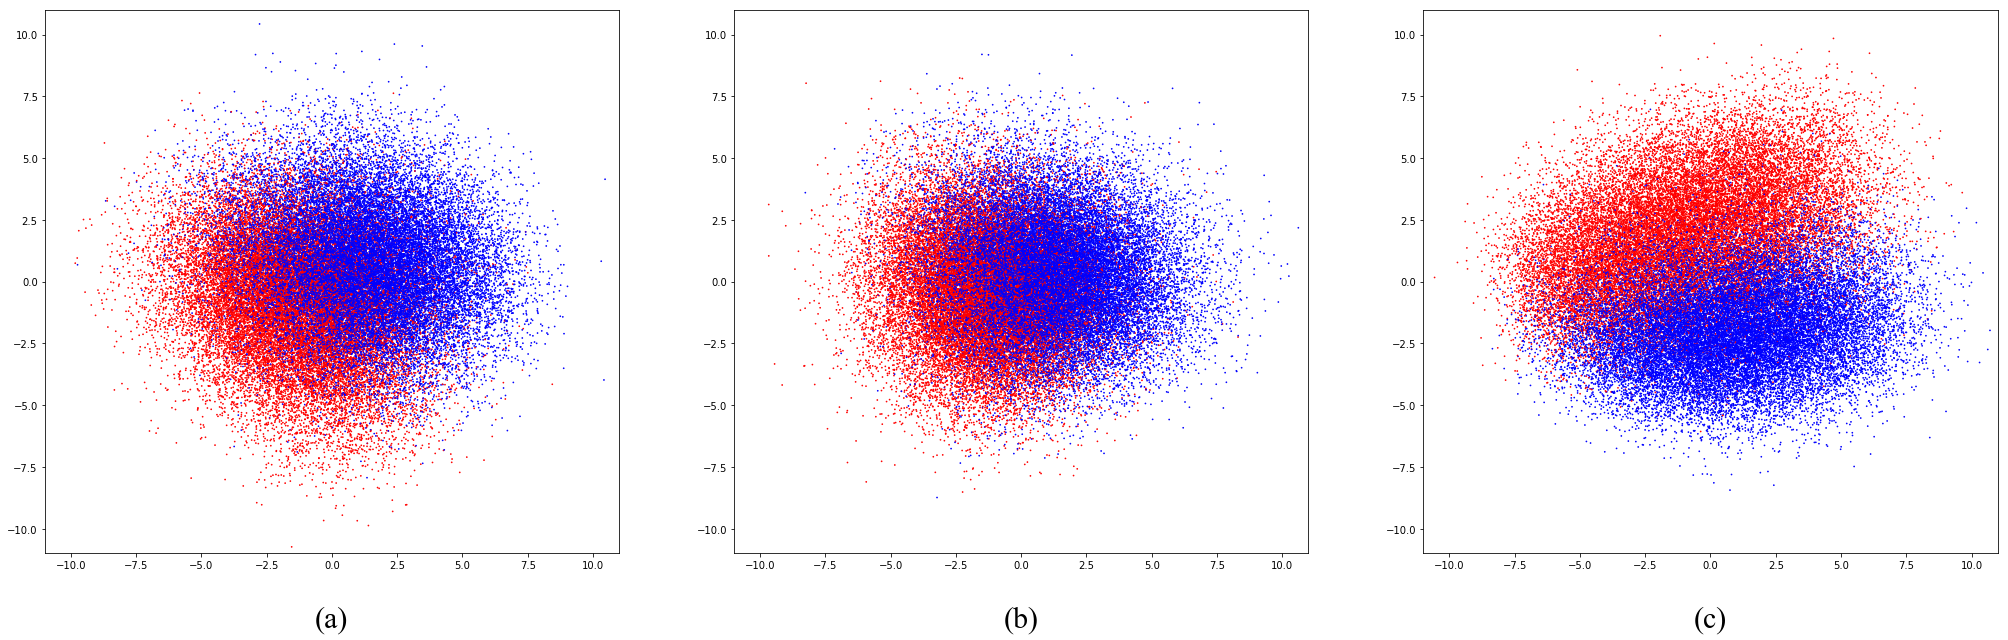
\includegraphics[width=\linewidth]{plot.png}
\caption{PCA visualization of embeddings trained with (a) dot product, (b) L2R dot product and (c) cos. similarity.}
\label{plot}
\end{figure*}

Grid search was performed using 20\% of the training data as a validation set in order to determine the optimal hyperparameters as well as whether to use a constant learning rate or learning rate annealing. Table~\ref{oph} shows the optimal hyperparameters for the models on the IMDB dataset. We did not tune the $N$ hyperparameter or the negative sampling size and left it the same as in \cite{li2016a} and \cite{lau2016}. We did however tune the number of iterations from [10, 20, 40, 80, 120], learning rate from [0.25, 0.025, 0.0025, 0.001] and $\alpha$ from [4, 6, 8]. A sensible value of $\alpha$ should be around 6, since looking at the graph of the sigmoid function, for input values
greater than 6 and less than -6, the sigmoid function doesn't change much and has values of close to 1 and 0, respectively. In the case of using L2 regularized dot product, $\lambda$ (regularization strength) was chosen from [1, 0.1, 0.01].

\begin{table}[h]
	\centering
	\small
	\begin{tabular}{@{\hskip6pt}lrrr@{\hskip6pt}}
		\toprule
					Hyperparameter 			& Dot 	&  L2R Dot 		& Cos.  \\ 
											& Prod. & Prod.  		&Sim. 	\\
		\midrule                                                            
					$N$ (dimensionality) 	& 500	& 500 			& 500 	\\
					Neg. Sampling Size 		& 5		& 5 			& 5 	\\
					Iterations 				& 10	& 20 			& 120 	\\ 
					Learning Rate 			&  0.25	& 0.025 		& 0.001 \\
					$\alpha$ 				& - 	& - 			& 6 	\\
					$\lambda$ 				& - 	& 0.01 			&- 		\\
					LR annealing &  true& false & false \\
		\bottomrule
	\end{tabular}
	\caption{Optimal Hyperparameters.}
	\label{oph}
\end{table}

The optimal learning rate in the case of cosine similarity is extremely small, suggesting a chaotic error surface. Since the learning rate is already small to begin with, no learning rate annealing  is used. The model in turn requires a larger number of epochs for convergence. For the distribution for sampling negative words, we used the n-gram distribution raised to the 3/4\textsuperscript{th} power in accordance with \cite{mikolov2013}. The weights of the networks were initialized from a uniform distribution in the range of [-0.001, 0.001]. 

\subsection{Results}

Each experiment was carried out 5 times and the mean accuracy is reported in Table~\ref{er}. This is to account for random factors such as shuffling document and word ids, and random initialization. From here we see that using cosine similarity instead of dot product improves accuracy across the board. The results are most apparent in the case of unigrams + bigrams. However it is not to suggest that switching from dot product to cosine similarity alone improves accuracy as other minor adjustments and hyperparameter tuning as explained was done. However it may imply that using cosine similarity allows for a higher potential accuracy as was achieved in these experiments. 

Regardless, we believe the comparisons are fair since each model is using its own set of optimal 
hyperparameters, but for the full sake of comparison, leaving everything the same and only switching out
dot product for cosine similarity ($\alpha$ = 1) as well as switching it out and using a sensible value of $\alpha$
at $\alpha$ = 6 both achieve an accuracy of around 50\%. This is because our model fails whenever the learning
rate is too large. As seen during grid search, whenever the initial learning rate was 0.25,
accuracy was always poor. 

Introducing L2 regularization to dot product improves accuracy for all cases except a depreciation in the case of using unigrams only, lucikily cosine similarity does not suffer from this same depreciation.  





\subsection{Discussion}

From table~\ref{es}, the mean Euclidean norm of embeddings trained with cosine similarity is lower than that of L2R dot product which is in turn lower than in the case of using dot product; this suggests that the method employing cosine similarity acts as a regularization mechanism, preventing the weights from getting too large. Large magnitudes of document vectors may be harder for the end classifier to fit in such a way that generalizes well, which may be why cosine similarity and L2R dot product perform better than dot product on the
IMDB dataset. 

As predicted, the mean cosine similarity between all pairs of vectors in the same class (Same Mean Cos. Sim.) is higher in the case of cosine similarity than the other two models. Unfortunately, the mean for all pairs in different classes (Diff. Mean Cos. Sim.) is higher as well. Further analysis and hopefully some formalism as to why cosine similarity performs better is a planned future work.

\begin{table}[h]
	\centering
	\small
	\begin{tabular}{@{\hskip6pt}lrrr@{\hskip6pt}}
		\toprule
		Embedding & Dot  &  L2R Dot &  Cos. \\ 
		Statistic&Prod.  & Prod.  & Sim. \\
		\midrule
		Same Mean Cos. Sim. & 0.23 & 0.20 & 0.35\\
		Diff. Mean Cos. Sim. & 0.21 & 0.17 & 0.32\\ 
		Mean Norm & 8.91 & 6.30 & 5.35\\
		\bottomrule
	\end{tabular}
	\caption{Embedding statistics.}
	\label{es}
\end{table}

Figure~\ref{plot} shows the projection of the embeddings along their first two principle components, different colors corresponding to different classes. Cosine similarity shows slightly better seperability between the two classes, while dot product and L2R dot product are quite similar.

\subsection{Feature Combination}

Another contribution of this paper is demonstrating the effectiveness of concatenating naive bayes weighted bag of n-grams with DV-ngram, L2R dot product, or document vectors trained with cosine similarity, the last achieving state of the art accuracy on the IMDB dataset. We note that all models utilize unigrams to trigrams and additional unlabeled data if possible. 
Table \ref{mc} shows a comparison between our
proposed models (shown in bold) and previous
state of the arts and other published results. 

\begin{table}[h]
	\centering
	\small
	\begin{tabular}{@{\hskip6pt}lr@{\hskip6pt}}
		\toprule
		Model & IMDB Dataset \\ 
		 & Accuracy (\%)\\
		\midrule
		NB-SVM Bigrams & 91.22  \\
		 \cite{wang2012}	& \\
		NB-SVM Trigrams & 91.87 \\
		\cite{mesnil2015} & \\
		DV-ngram  & 92.14 \\
		\cite{li2016a} & \\
		\bf{Dot Product with} & \bf{92.45} \\
		\bf{L2 Regularization} & \\ 
		Paragraph Vector & 92.58 \\
		\cite{le2014} & \\
		\bf{Document Vectors using} & \bf{93.13} \\
		\bf{Cosine Similarity} & \\
		W-Neural-BON Ensemble & 93.51 \\
		\cite{li2016b} & \\
		TGNR Ensemble & 93.51 \\
		\cite{li2017} & \\
		TopicRNN & 93.76 \\
		\cite{dieng2017} & \\
		One-hot bi-LSTM & 94.06 \\
		\cite{johnson2016} \\
		Virtual Adversarial & 94.09 \\
		\cite{miyato2016} & \\
		BERT large finetune UDA & 95.80\\
		\cite{xie2019} & \\
		\bf{NB-weighted-BON +} & \bf{96.95} \\
		\bf{DV-ngram} & \\
		\bf{NB-weighted-BON +} & \bf{97.17} \\
		\bf{L2R Dot Product} & \\
		\bf{NB-weighted-BON +} & \bf{97.42} \\
		\bf{Cosine Similarity} & \\
		\bottomrule
	\end{tabular}
	\caption{Comparison with other models.}
	\label{mc}
\end{table}

\section{Conclusion and Future Work}

Our proposed model trains document embeddings using cosine similarity as the similarity measure and we show that sentiment classification performance on the IMDB dataset is improved when utilizing these embeddings as opposed to those trained using dot-product. Cosine similarity may help reduce overfitting to the embedding task, and this regularization in turn produces more useful embeddings. We also show that concatenating these embeddings with Naïve bayes weighed bag of n-grams results in high accuracy on the IMDB dataset. 

 An important future development is to carry out experiments on other datasets. It is essential that we benchmark on more than one dataset, to prevent superficially good results by overfitting hyperparameters or the cosine similarity model itself to  the IMDB dataset. 
Other tasks and datasets include: (1) sentiment analysis - the Stanford sentiment treebank dataset \cite{socher2013}, the polarity dataset v2.0 \cite{pang2004}, (2) topic classification -  AthR, XGraph, BbCrypt \cite{wang2012}, and (3) semantic relatedness tasks - datasets from the SemEval semantic textual similarity (STS) tasks \cite{agirre2015}.





\bibliography{acl2019}
\bibliographystyle{acl_natbib}

\appendix

\section{Obtaining the weight update equations in the case of cosine similarity}

To obtain the weight update equations for the input and output vectors of our model in each iteration of stochastic gradient descent, we must find the gradient of the error function at a given training example, which may be considered a document, n-gram pair. 

Let: 
\begin{align}
E =  &- \log \sigma \left( \alpha \cos \theta_{w_o} \right) \nonumber \\
&- \sum_{w_n \in W_{neg}} \log \sigma \left( - \alpha \cos \theta_{w_n} \right)  
\end{align}
where:
\begin{equation}
\cos \theta_w = \frac {\mathbold{v}_d^T \mathbold{v}_w} {\lVert \mathbold{v}_d \rVert \lVert \mathbold{v}_w \rVert}
\end{equation}
be the objective function at a single training example $(d,w_o)$. Then, to find the gradient of $E$ first differentiate $E$ with respect to $\cos \theta_w$: 
\begin{equation}
\frac {\partial E} {\partial \cos \theta_w} = \alpha \left( \sigma \left( \alpha \cos \theta_w \right) - t \right)
\end{equation}
where $t = 1$ if $w = w_o$; $0$ otherwise. We then obtain the derivative of $E$ w.r.t. the output n-gram vectors: 
\begin{equation}
\frac {\partial E} {\partial \mathbold{v}_w} = \frac {\partial E} {\partial \cos \theta_w} \cdot \frac {\partial \cos \theta_w} {\partial \mathbold{v}_w} 
\end{equation}
\begin{align}
\frac {\partial E} {\partial \mathbold{v}_w} = {}&\alpha \left( \sigma \left( \alpha \cos \theta_w \right) - t \right) \nonumber \\
&\cdot\left( \frac {\mathbold{v}_d} {\lVert \mathbold{v}_d \rVert \lVert \mathbold{v}_w \rVert} - \frac { \mathbold{v}_w\left(\mathbold{v}_d^T \mathbold{v}_w\right)} {\lVert \mathbold{v}_d \rVert \lVert \mathbold{v}_w \rVert^3} \right)
\end{align}

This leads to the following weight update equation for the output vectors: 
\begin{equation}
\mathbold{v}_w^{(new)} = \mathbold{v}_w^{(old)} - \eta \frac {\partial E} {\partial \mathbold{v}_w}
\end{equation}
where $\eta$ is the learning rate. This equation needs to be applied to all $w \in \{w_o\} \cup W_{neg}$ in each iteration.

Next, the errors are backpropagated and the input document vectors are updated. Differentiating $E$ with respect to $\mathbold{v}_d$: 
\begin{equation}
\frac {\partial E} {\partial \mathbold{v}_d} = \sum_{w \in \{w_o\} \cup W_{neg}}  \frac {\partial E} {\partial \cos \theta_w} \cdot \frac {\partial \cos \theta_w} {\partial \mathbold{v}_d}
\end{equation}
\begin{align}
{}= \sum_{\mathclap{w \in \{w_o\} \cup W_{neg}}}{} &\alpha \left( \sigma \left( \alpha \cos \theta_w \right) - t \right) \nonumber \\
&\cdot\left( \frac {\mathbold{v}_w} {\lVert \mathbold{v}_d \rVert \lVert \mathbold{v}_w \rVert} - \frac { \mathbold{v}_d\left(\mathbold{v}_d^T \mathbold{v}_w\right)} {\lVert \mathbold{v}_d \rVert^3 \lVert \mathbold{v}_w \rVert} \right)
\end{align}

Thus, we obtain the weight update equation for the input vector in each iteration: 
\begin{equation}
\mathbold{v}_d^{(new)} = \mathbold{v}_d^{(old)} - \eta \frac {\partial E} {\partial \mathbold{v}_d}
\end{equation}

\section{Weight update equations in the case of dot product}
This section contains the weight update equations for the input and output vectors of the dot product model in each iteration of stochastic gradient descent.

The following weight update equations for the output vectors:
\begin{equation}
\mathbold{v}_w^{(new)} = \mathbold{v}_w^{(old)} - \eta \left( \sigma \left( \mathbold{v}_d^T \mathbold{v}_w \right) - t \right) \cdot \mathbold{v}_d
\end{equation}
where $t = 1$ if $w = w_o$; $0$ otherwise, needs to be applied to all $w \in \{w_o\} \cup W_{neg}$ in each iteration.

The following weight update equation needs to be applied to the input vector in each iteration:
\begin{equation}
\mathbold{v}_d^{(new)} = \mathbold{v}_d^{(old)} - \eta \sum_{\mathclap{w \in \{w_o\} \cup W_{neg}}} \left( \sigma \left( \mathbold{v}_d^T \mathbold{v}_w \right) - t \right) \cdot \mathbold{v}_w
\end{equation}

\section{Weight update equations in the case of L2R dot product}
This section contains the weight update equations for the input and output vectors of the L2R dot product model in each iteration of stochastic gradient descent.

The following weight update equations for the output vectors:
\begin{align}
\mathbold{v}_w^{(new)} = \mathbold{v}_w^{(old)} &- \eta \left( \sigma \left( \mathbold{v}_d^T \mathbold{v}_w \right) - t \right) \cdot \mathbold{v}_d \nonumber \\
&- \eta \lambda \mathbold{v}_w
\end{align}
where $t = 1$ if $w = w_o$; $0$ otherwise, needs to be applied to all $w \in \{w_o\} \cup W_{neg}$ in each iteration.

The following weight update equation needs to be applied to the input vector in each iteration:
\begin{align}
\mathbold{v}_d^{(new)} = \mathbold{v}_d^{(old)} &- \eta \sum_{\mathclap{w \in \{w_o\} \cup W_{neg}}} \left( \sigma \left( \mathbold{v}_d^T \mathbold{v}_w \right) - t \right) \cdot \mathbold{v}_w \nonumber \\
&- \eta \lambda \mathbold{v}_d
\end{align}


\end{document}
